\subsection{Analyse der generierten XML-Berichte und bestehenden Strukturen}
\label{subsec:analyse-der-generierten-xml-berichte-und-bestehenden-strukturen}

In diesem Unterkapitel wird der Aufbau der automatisch
generierten Testberichte aus dem Teststand und der vorhandenen Ausgabe- und Speicherstruktur
erläutert. Dies ist relevant für die Erstellung der Datenbank und das
Verständnis der Ein- und Auslesefunktionen der Web-Applikation.

\subsubsection{XML-Berichtsstrukturschema}

Die vom Teststand automatisch generierten
Berichte folgen einem konstanten Strukturschema, welches sich bis zu einer
gewissen Ebene der XM-Struktur in jedem Bericht wiederholt. Wie im Kapitel „Grundlagen“
beschrieben, kann ein Element Attribute, andere Elemente und einen Inhaltswert beinhalten.

Das Stammelement heißt in allen automatisch
generierten Berichten „test“ und besitzt immer das Attribut „id“. Die Zahl in
diesem Attribut beschreibt den Typ des \ac{DUTs} die in diesem Test geprüft wurden.

Das Stammelement hat die Unter- bzw.
Kinderelemente „info“, „testbench“, „string“ und dreimal „testmodule“.
Diese Elemente haben wiederum alle weiter Unterelemente und Attribute.
In der folgenden Abbildung \ref{fig: Aufbau unferänderlicher XML-Berichtstruktur} ist die unveränderliche Struktur eines Testberichtes abgebildet, welcher erfolgreich durchgeführt wurde.

\begin{figure}[H]
    \centering
    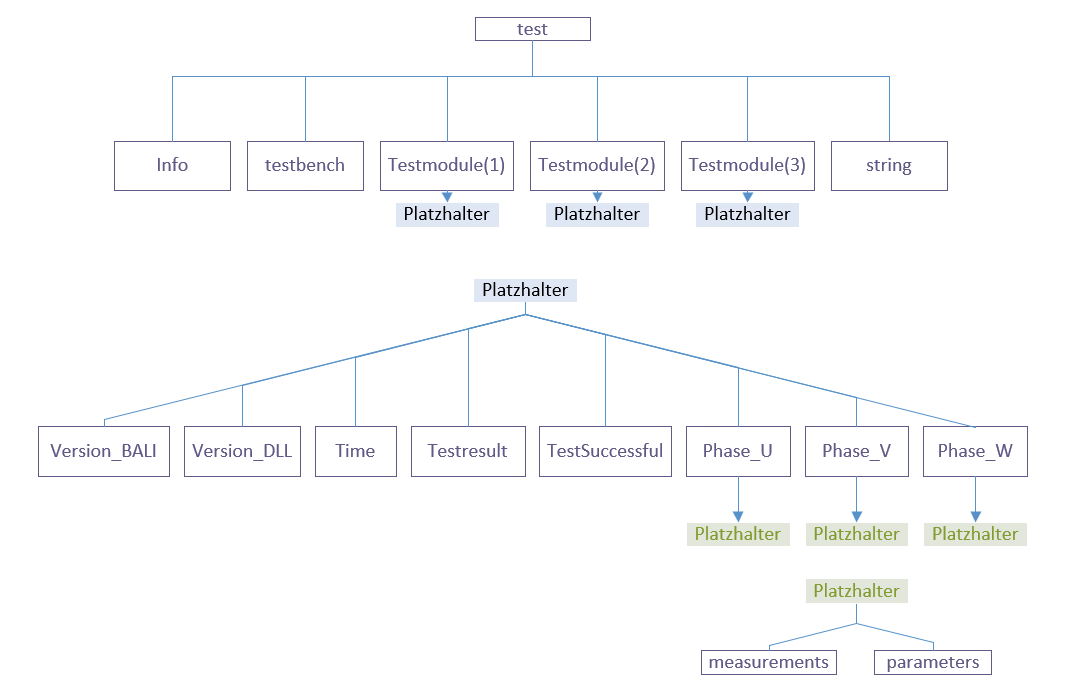
\includegraphics[width=0.95\textwidth]{Grafiken/XML-Strukturdiagramm}
    \caption{Aufbau unferänderlicher XML-Berichtstruktur}
    \label{fig: Aufbau unferänderlicher XML-Berichtstruktur}
    {Quelle: Eigene Darstellung mit Microsoft Visio}
\end{figure}

Hierbei sollte angemerkt werden, dass in allen Testberichten die Elemente, die kein Unterelement besitzen gleich aufgebaut sind.
Sie besitzen mindestens das Attribut „name“ und ihre Elementenbezeichnung ist immer nach dem Datentyp ihres Inhalts benannt.
Für ein besseres Verständnis siehe Abbildung \ref{fig: Elementaufbau aus XML-Bericht}.


\begin{figure}[H]
    \centering
    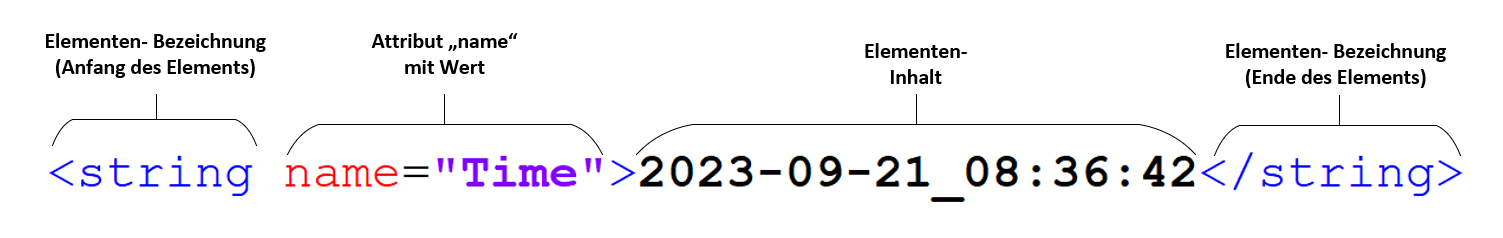
\includegraphics[width=0.95\textwidth]{Grafiken/Elementaufbau}
    \caption{Elementaufbau aus XML-Bericht}
    \label{fig: Elementaufbau aus XML-Bericht}
    {Quelle: Eigene Darstellung mit Microsoft Visio}
\end{figure}

Jedes der Elemente „testmodule“ hat ein Attribut
„name“, durch welches Sie unterschieden werden können. Das Element „string“ hat
ein Namensattribut mit der Bezeichnung „test sequence status“. Der Inhalt
dieses Elementes gibt an, ob der Test erfolgreich abgeschlossen wurde oder ob
es einen Fehler bzw. eine Grenzüberschreitung von Messwerten gab.
Die hier genannten eigenschaften sind in der Abbildung \ref{fig: Direkte Kinderelement unter Stammelement} zu erkennen.

\begin{figure}[H]
\centering
\begin{minipage}{0.95\textwidth}
\begin{lstlisting}[language=XML]
<?xml version="1.0" encoding="UTF-8"?>
    <test id="124">
    <info></info>
    <testbench></testbench>
    <testmodule name="DriverConsumptionTest"></testmodule>
    <testmodule name="PulseTest FSW L"></testmodule>
    <testmodule name="XPowerTest"></testmodule>
    <string name="test sequence status">
        Test sequence successfully finished.</string>
    </test>
\end{lstlisting}
\end{minipage}
\caption{Direkte Kinderelement unter Stammelement}
\label{fig: Direkte Kinderelement unter Stammelement}
    {Quelle: Eigene Darstellung}
\end{figure}


Das Element „info“ enthält in seinen Unterelementen die allgemeinen Testinformationen, wie die Startzeit des Tests,
die Typen-ID, die Konfigurationsbezeichnung des Teststandes, die Bezeichnung des angeschlossenen Carriers und die
Seriennummern des \ac{DUTs}. Diese Elemente haben keine Unterelemente und sind alle mit einem Namensattribut und einem Inhalt definiert.
Für die genauen Bezeichnungen und Struktur siehe Abbildung \ref{fig: XML-Strukturbeispiel Info-Element}

\begin{figure}[H]
\centering
\begin{minipage}{0.95\textwidth}
\begin{lstlisting}[language=XML]
<info>
	<string name="Time">2023-09-21_08:36:33</string>
	<string name="Material_number">124</string>
	<string name="Configuration">L_3DUT_3P1Q</string>
	<string name="ID_Carrier_left">Carrier 1</string>
	<string name="ID_DUT_R">10-29550</string>
	<string name="ID_DUT_S">10-29396</string>
        <string name="ID_DUT_T">10-29482</string>
</info>
\end{lstlisting}
\end{minipage}
\caption{XML-Strukturbeispiel Info-Element}
\label{fig: XML-Strukturbeispiel Info-Element}
    {Quelle: Eigene Darstellung}
\end{figure}

Die Teststandbezeichnung und die Versionen der Hard- und Software werden im Element „testbench“ gespeichert.
Diese Elemente enthalten auch keine weiteren Unterelemente und sind alle mit einem Namensattribut und einem Inhalt versehen.
Die genauen Bezeichnungen und die Struktur sind in Abbildung \ref{fig: XML-Strukturbeispiel Testbench-Element} zu sehen.

\begin{figure}[H]
\centering
\begin{minipage}{0.95\textwidth}
\begin{lstlisting}[language=XML]
<testbench>
	<string name="Testbench_name">USTB_DtWind</string>
	<string name="Testbench_HW_revision">V1.5</string>
	<string name="Version_GUI">V1.4.1</string>
        <string name="Version_controller">V1.3.2</string>
</testbench>
\end{lstlisting}
\end{minipage}
\caption{XML-Strukturbeispiel Testbench-Element}
\label{fig: XML-Strukturbeispiel Testbench-Element}
    {Quelle: Eigene Darstellung}
\end{figure}


Die Testmodule-Elemente sind alle nach dem gleichen Schema aufgebaut. Die ersten Unterelemente enthalten Grundinformationen
zu dem Status des Testmoduls, der Tages- und Uhrzeit des Tests und welche Versionen davon verwendet wurden.
Danach befinden sich noch drei weitere Elemente im Element „module“.
Diese Elemente heißen „Phase U“, „Phase V“ und „Phase W“.
Sie besitzen kein Namensattribut, siehe Abblidung \ref{fig: XML-Strukturbeispiel Testmodulheader}.

\begin{figure}[H]
\centering
\begin{minipage}{0.95\textwidth}
\begin{lstlisting}[language=XML]
<testmodule name="DriverConsumptionTest">
	<integer name="TestSuccessful" min="1" max="1">1</integer>
	<string name="Testresult">
        Test finished successfully!</string>
	<string name="Time">2023-09-21_08:36:42</string>
	<string name="Version_DLL">V1.2.4</string>
	<string name="Version_BALI">V1.2.4</string>
    <Phase_U>...</Phase_U>
    <Phase_V>...</Phase_V>
    <Phase_W>...</Phase_W>
</testmodule>
\end{lstlisting}
\end{minipage}
\caption{XML-Strukturbeispiel Testmodulheader}
\label{fig: XML-Strukturbeispiel Testmodulheader}
    {Quelle: Eigene Darstellung}
\end{figure}

Diese Phasenelemente enthalten die Parameter und die Messdaten für die DUTs. Jede Phase enthält die Messwerte für ein DUT.
Somit besitzen alle Module unter dem Element „Phase U“ die Messwerte und Parameter für den ersten DUT, dessen Seriennummer
unter dem Element mit dem Namensattribut „ID DUT R“ in Abbildung \ref{fig: XML-Strukturbeispiel Info-Element} zu finden ist.

In dem Element „parameters“, welches in jedem Phasenelement vorkommt, befinden sich die voreingestellten Rahmbedingungen
und Anforderungen für das Testmodul. Diese enthalten alle ein Namensattribut und einen Inhalt.

Die Elemente unter dem Eintrag „measurements“ enthalten die Messdaten der Testmodule. Sie haben oft noch extra Attribute
wie „min“ oder „max“, welche die Toleranzgrenzen beschreiben. Diese Toleranzgrenzen zeigen, in welchem Bereich der jeweilige
Elementinhalt angesiedelt sein muss, um kein positives bzw. fehlerfreies Ergebnis zu erzeugen.
Die meisten Attributswerte finden sich schon in den Parametern wieder und sind somit doppelt im Bericht zu finden.
Nur bei den Floatblock-Elementen, also Elementen mit der Bezeichnung Floatblock, sind besondere Attribute zu finden,
welche nicht gedoppelt vorkommen.
Diese Elemente umfassen zusätzlich die Attribute „size“ und „duration“, welche die Anzahl der in dem Inhalt enthaltenen
Floatwerte und die Dauer der Werteaufnahme angeben dies ist in Abbildung \ref{fig: Beispiel XPowertest Floatblock-Elemente} zu erkennen.
Diese sind für die grafische Darstellung besonders relevant.

\begin{figure}[H]
\centering
\begin{minipage}{0.95\textwidth}
\begin{lstlisting}[language=XML]
<floatblock name="Time" size="698" duration="959.952" unit="s">
0.71365,2.1370,3.5323,...</floatblock>
\end{lstlisting}
\end{minipage}
\caption{Beispiel XPowertest Floatblock-Elemente}
\label{fig: Beispiel XPowertest Floatblock-Elemente}
    {Quelle: Eigene Darstellung}
\end{figure}

Auf der Phasenebene treten keine Veränderungen in der \ac{XML}-Struktur auf, variieren lediglich die Elemente unter den
Phasenelementen von Bericht zu Bericht etwas.
Die beträchtliche Ausnahme von dieser Regel bilden die Berichte, bei denen ein Fehler aufgetreten ist oder sogar der
Testvorgang abgebrochen wurde. Bei diesen Berichten hört die \ac{XML}-Struktur bei den fehlgeschlagenen Testmodulen schon auf.
Der Testbericht ist aber in sich geschlossen. Das bedeutet, die \ac{XML}-Struktur ist vollkommen und kann von einem \ac{XML}-Parser eingelesen werden.
Es befinden sich nur weniger Testmodul-Elemente in dem Bericht und im Element für den Testsequenzstatus ist folgender Inhalt
enthalten „Test sequence finished with errors“. Zudem wird bei dem Testmodul, bei dem der Fehler aufgetreten ist, unter
dem Element mit dem Namen „Testresult“ ein Fehlercode und seine Bedeutung ausgegeben. In Abbildung \ref{fig: Beispiel Fehler bei DriverConsumptionTest} ist ein
Beispiel für einen Bericht, welcher beim ersten Testmodul einen Fehler ausgegeben hatte.
Bei einem Ausfall eines der zu testenden \ac{DUTs} gibt es die Besonderheit, dass die anderen noch funktionsfähigen \ac{DUTs}
keine weiteren Datenaufnahmen mehr machen können. Denn das System benötigt alle drei Phasen, um den Test durchzuführen.
Die \ac{XML}-Struktur ist in sich geschlossen, aber es werden keine Daten von den anderen \ac{DUTs} mehr aufgenommen.

\begin{figure}[H]
\centering
\begin{minipage}{0.95\textwidth}
\begin{lstlisting}[language=XML]
<testmodule name="DriverConsumptionTest">
	<integer name="TestSuccessful" min="1" max="1">0</integer>
	<string name="Testresult">Idrv not within limits on Phase U
0x30010019 !
0x30010013</string>
	<string name="Time">2021-03-10_09:10:37</string>
	<string name="Version_DLL">V1.2.4</string>
    <string name="Version_BALI">V1.2.4</string>
    <Phase_U>...</Phase_U>
    <Phase_V>...</Phase_V>
        <Phase_W>...</Phase_W>
</testmodule>
\end{lstlisting}
\end{minipage}
\caption{Beispiel Fehler bei DriverConsumptionTest}
\label{fig: Beispiel Fehler bei DriverConsumptionTest}
    {Quelle: Eigene Darstellung}
\end{figure}





